
\section{Elementos Visuais}
O projeto bebe de variadas fontes de inspirações, e planeja levar o jogador para o ambiente em que os personagem que ele irá controlar vivem, finalizando em outro ambiente que misturará elementos de todos os ambientes.


Todos os personagens foram baseados em estatuetas artesanais, desenhados em 2D e por fim modelados em 3D.

\subsection{Duende}
\subsubsection{Ambiente}
O ambiente do duende, Fulkominn, foi inspirado na Vila de Geiranger, e a partir de imagens dela geramos uma palheta de cores principais para o cenário.

\begin{figure}[htb]
	\caption{\label{fig_palhetaFulkominn}Palheta de Cores Fulkominn}
	\begin{center}
	    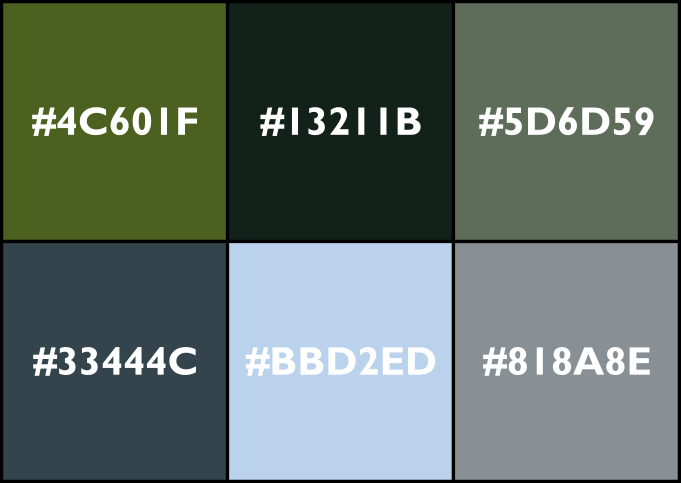
\includegraphics[width=\textwidth/2]{imagens/PaletaGeiranger.png}
	\end{center}
	\legend{Fonte: Autoria Nossa}
\end{figure}

\subsubsection{Personagem}

\begin{figure}[htb]
	\caption{\label{duendeRef}Estatueta de Duende}
	\begin{center}
	    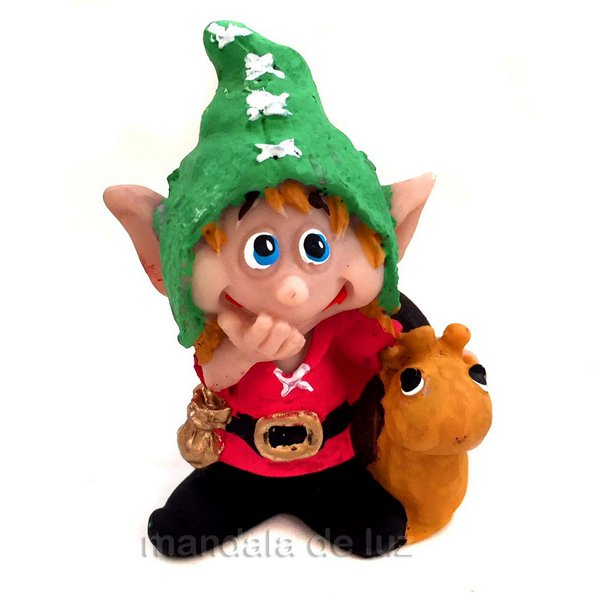
\includegraphics[width=\textwidth/2]{imagens/duendeRef.jpg}
	\end{center}
	\legend{Fonte: (Mandala de Luz, 2012)}
\end{figure}



\begin{figure}[htb]
	\caption{\label{duendePos}Arte Conceitual Duende}
	\begin{center}
	    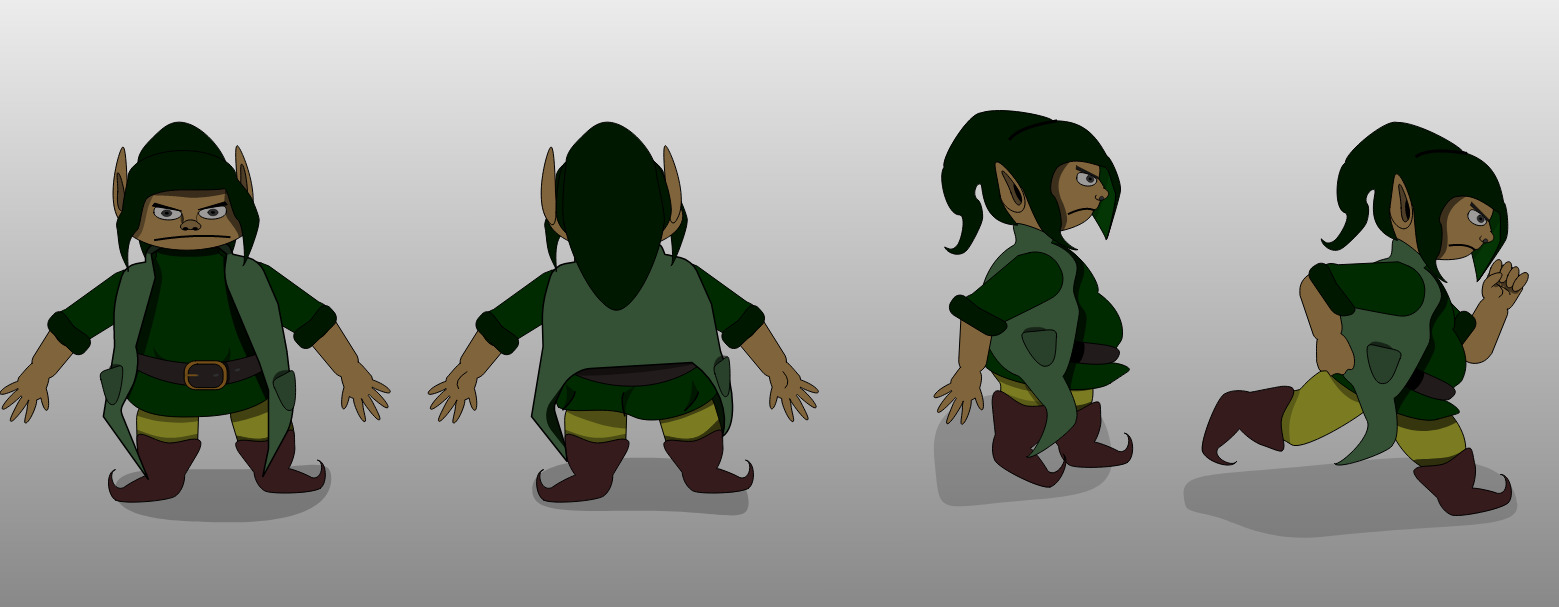
\includegraphics[width=\textwidth]{imagens/duendePosicoes.jpeg}
	\end{center}
	\legend{Fonte: Autoria Própria - Marina Araujo}
\end{figure}

\clearpage

\subsection{Xamã}

\subsubsection{Ambiente}
O ambiente do Xamã foi inspirado no parque nacional de Mesa Verde nos Estados Unidos, que é um sítio arqueológico com construções Pueblo.

\begin{figure}[htb]
	\caption{\label{fig_paletaMesa}Paleta de Cores Ambiente Xamã}
	\begin{center}
	    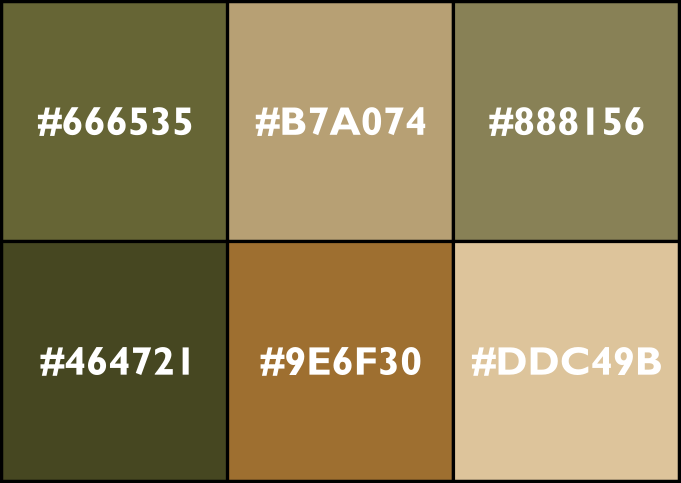
\includegraphics[width=\textwidth/2]{imagens/PaletaMesaVerde.png}
	\end{center}
	\legend{Fonte: Autoria Nossa}
\end{figure}




\subsubsection{Personagem}

\subsection{Bruxa}
\subsubsection{Ambiente}
O ambiente da Bruxa foi inspirado na vila de Killin do reino unido, e a palheta de cores principais pode ser observada na figura \ref{fig_paletaKilin}.

\clearpage

\begin{figure}[htb]
	\caption{\label{fig_paletaKilin}Paleta de Cores Ambiente Bruxa}
	\begin{center}
	    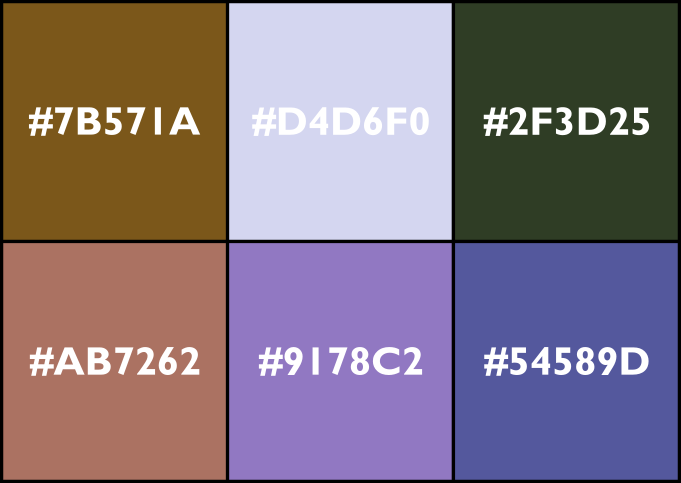
\includegraphics[width=\textwidth/2]{imagens/PaletaKilin.png}
	\end{center}
	\legend{Fonte: Autoria Nossa)}
\end{figure}

\subsubsection{Personagem}



\begin{figure}[htb]
	\caption{concept Bruxa}
	\begin{center}
	    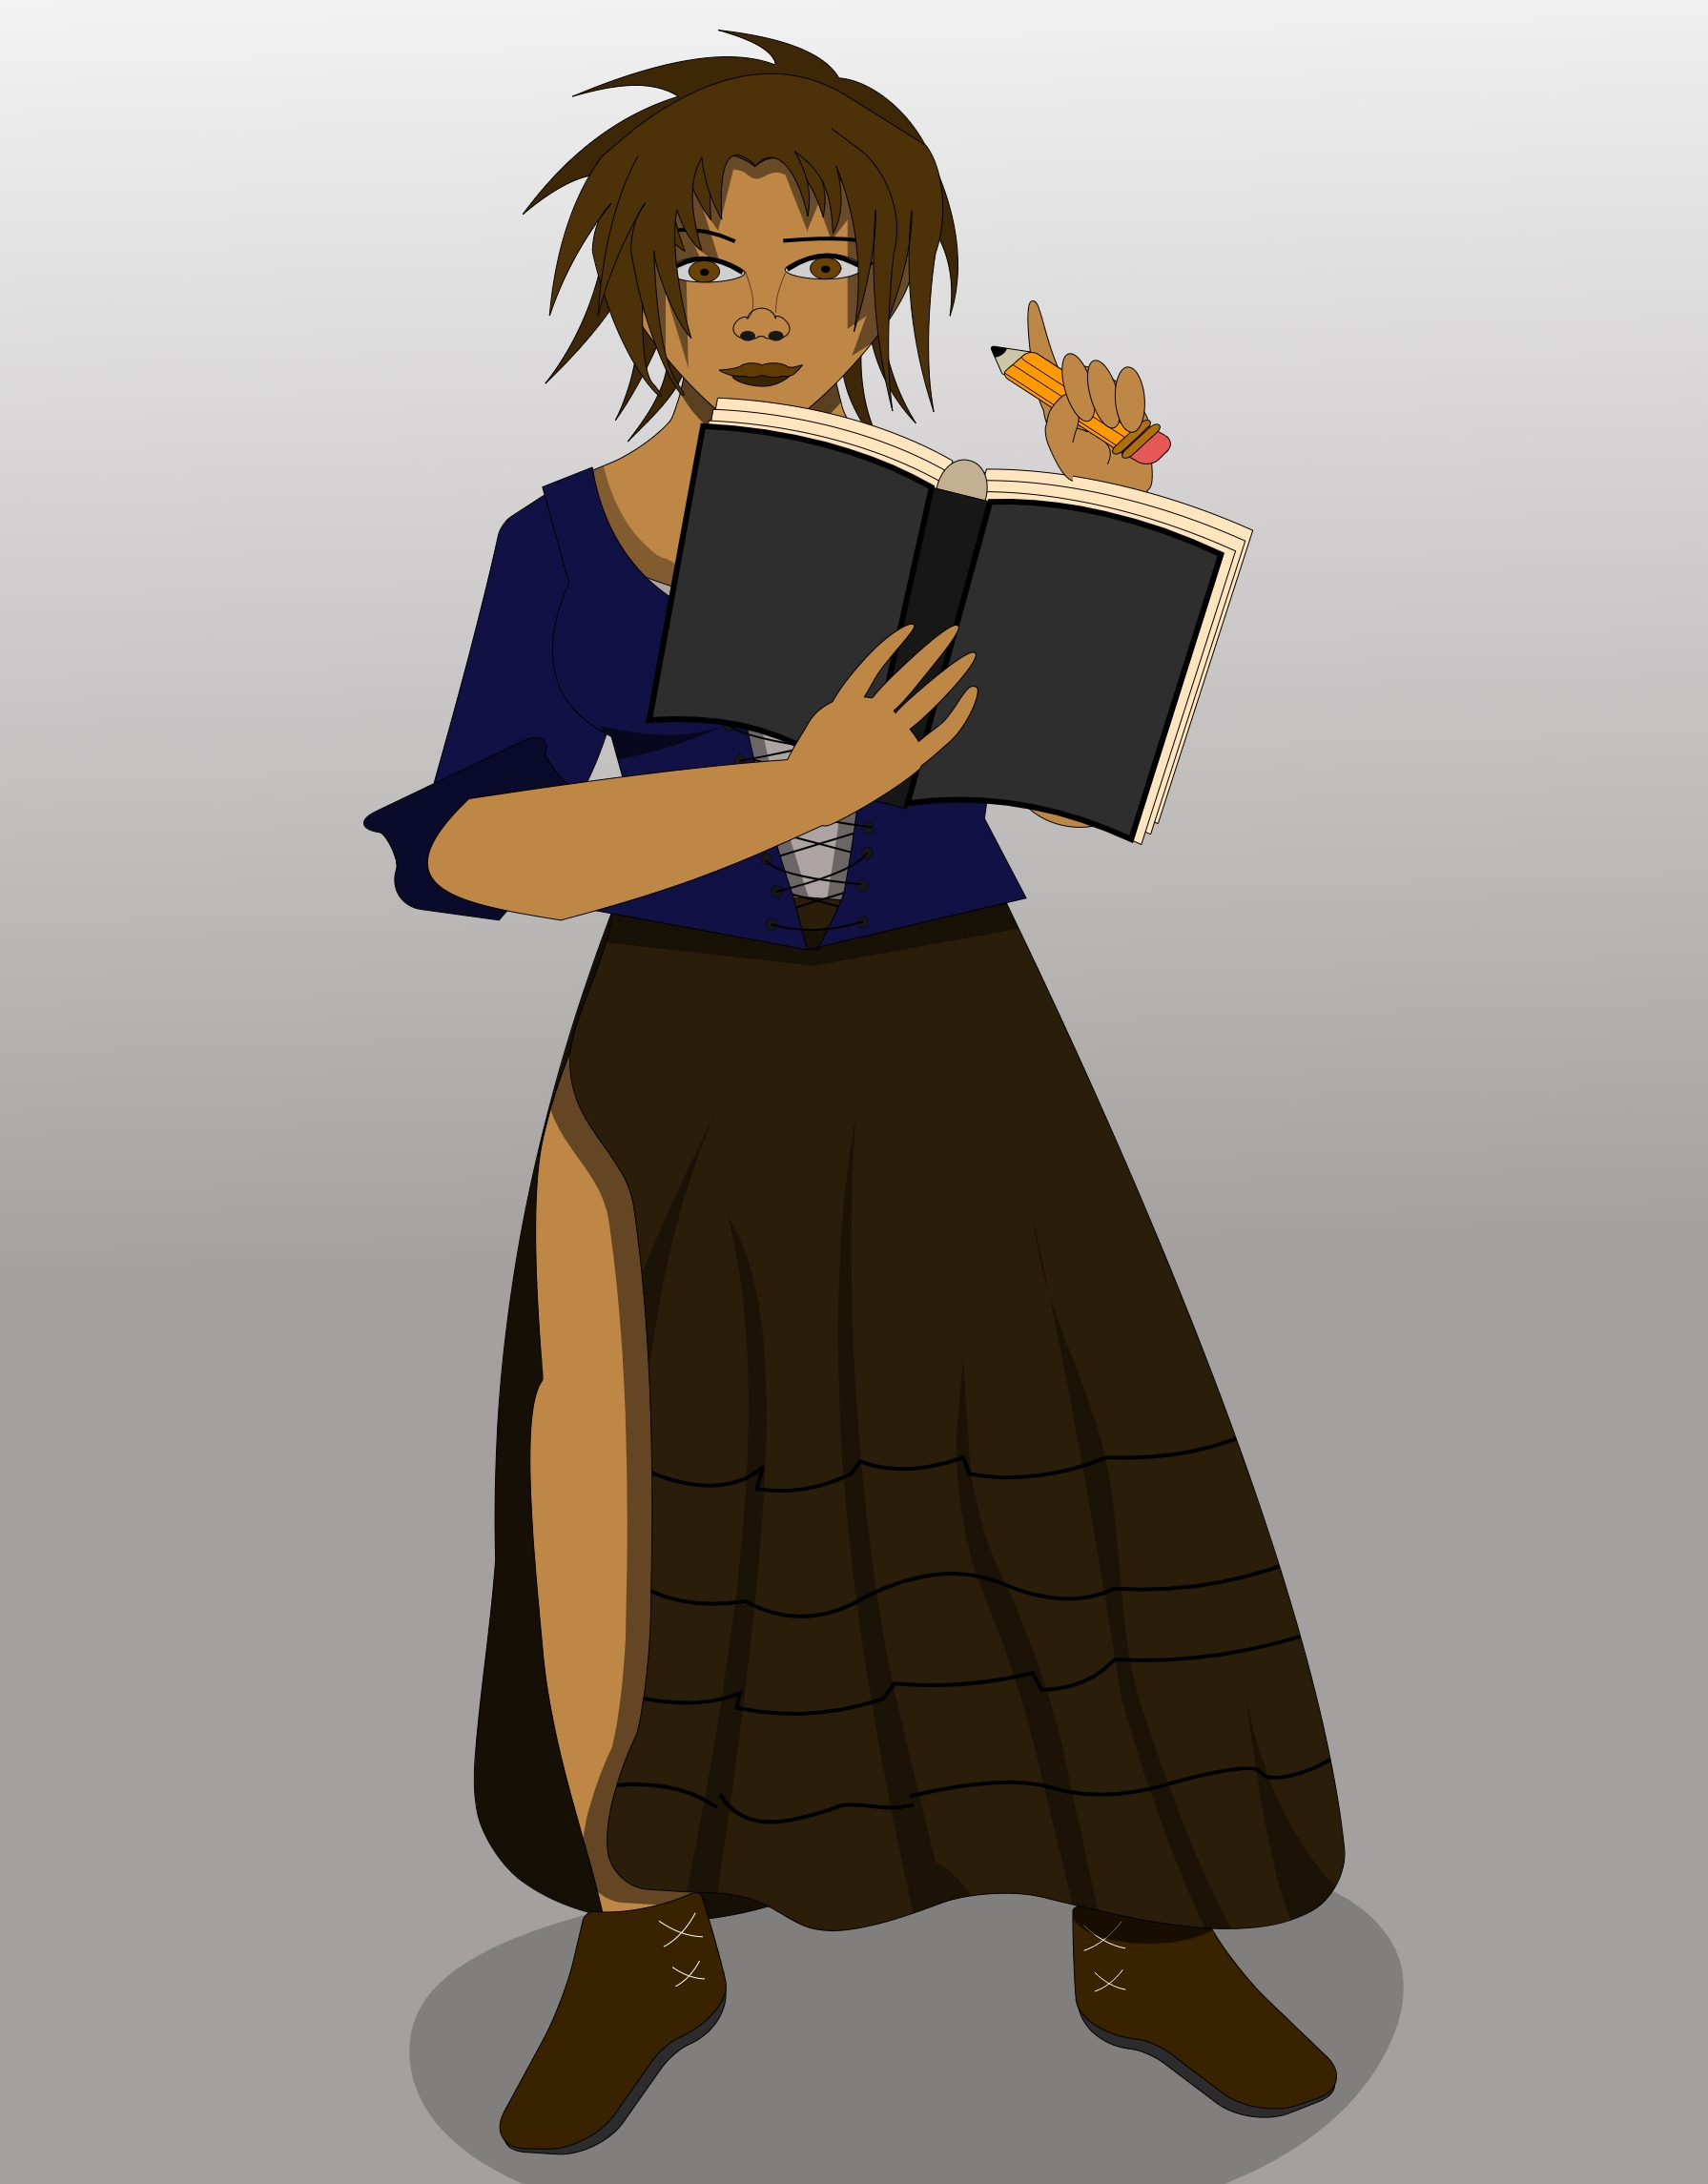
\includegraphics[width=\textwidth/2]{imagens/capaportifolio.jpeg}
	\end{center}
	\legend{Fonte: Autoria Nossa}
\end{figure}


\clearpage

\subsection{Ogof}
\begin{figure}[htb]
	\caption{\label{mago}mago}
	\begin{center}
	    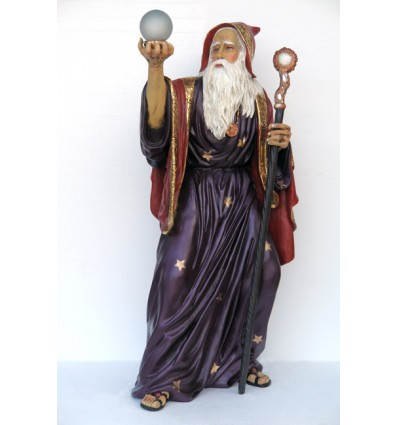
\includegraphics[width=\textwidth/2]{imagens/mago.jpg}
	\end{center}
	\legend{Fonte: (Macocaya, 2010)}
\end{figure}

\begin{figure}[htb]
	\caption{\label{Ogof}Ogof}
	\begin{center}
	    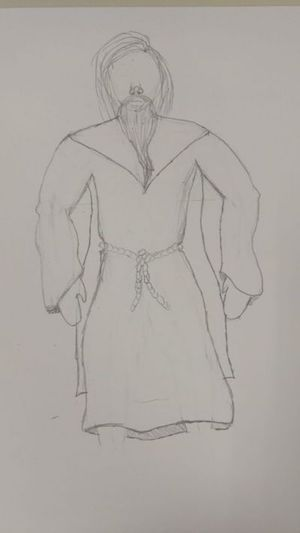
\includegraphics[width=\textwidth/2]{imagens/Ogof.jpg}
	\end{center}
	\legend{Fonte: Autoria Própria - Marina Araujo}
\end{figure}

\clearpage

\subsection{O Templo das Joias}

O Templo das Joias, foi inspirado em no parque Nacional de Tikal na Guatemala, onde estão templos da antiga cultura Maia.

\begin{figure}[htb]
	\caption{\label{fig_paletaTikal}Paleta de Cores Templo das Joias}
	\begin{center}
	    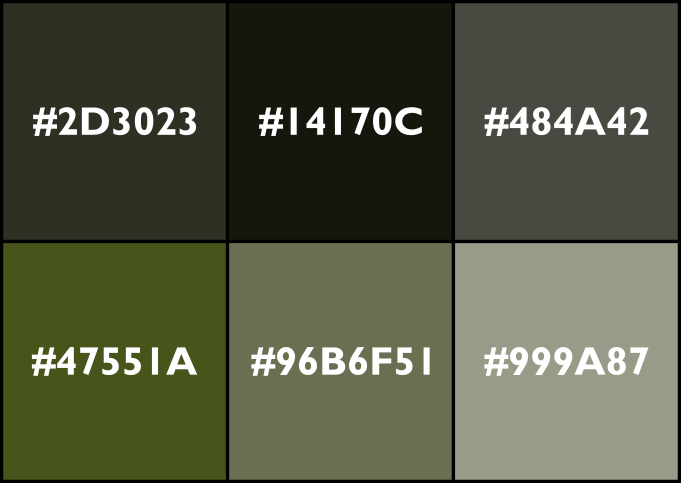
\includegraphics[width=\textwidth/2]{imagens/PaletaTikal.png}
	\end{center}
	\legend{Fonte: Autoria Nossa}
\end{figure}



\section{Elementos Sonoros}

Para uma maior imersão nos ambientes fantasticos que o jogo propoe, as trilha são inspiradas em músicas dos estilos \textit{new age, folk} e músicas tradicionais, nativo americanas, maia, entre outras.

Os elementos sonoros serão produzidos pela equipe, e também serão utilizados efeitos e musicas conseguidas na internet que tenha a licença Creative Commons, e serão dados os devidos créditos, tanto no guia impresso do jogo como nas de créditos.
